% Copyright 2004 by Till Tantau <tantau@users.sourceforge.net>.
%
% In principle, this file can be redistributed and/or modified under
% the terms of the GNU Public License, version 2.
%
% However, this file is supposed to be a template to be modified
% for your own needs. For this reason, if you use this file as a
% template and not specifically distribute it as part of a another
% package/program, I grant the extra permission to freely copy and
% modify this file as you see fit and even to delete this copyright
% notice. 

\documentclass[aspectratio=169, handout, 10pt, hyperref=colorlinks]{beamer}

% There are many different themes available for Beamer. A comprehensive
% list with examples is given here:
% http://deic.uab.es/~iblanes/beamer_gallery/index_by_theme.html
% You can uncomment the themes below if you would like to use a different
% one:
%\usetheme{AnnArbor}
%\usetheme{Antibes}
%\usetheme{Bergen}
%\usetheme{Berkeley}
%\usetheme{Berlin}
\usetheme{Boadilla}
%\usetheme{boxes}
%\usetheme{CambridgeUS}
%\usetheme{Copenhagen}
%\usetheme{Darmstadt}
%\usetheme{default}
%\usetheme{Frankfurt}
%\usetheme{Goettingen}
%\usetheme{Hannover}
%\usetheme{Ilmenau}
%\usetheme{JuanLesPins}
%\usetheme{Luebeck}
% \usetheme{Madrid}
%\usetheme{Malmoe}
%\usetheme{Marburg}
%\usetheme{Montpellier}
%\usetheme{PaloAlto}
%\usetheme{Pittsburgh}
%\usetheme{Rochester}
%\usetheme{Singapore}
%\usetheme{Szeged}
%\usetheme{Warsaw}

\title{Computational Commutative Algebra and Geometry}
% A subtitle is optional and this may be deleted
\subtitle{EE451 Supervised Research Exposition}

% \author{F.~Author\inst{1} \and S.~Another\inst{2}}
\author[Param Rathour]{Rathour Param Jitendrakumar\\190070049}
% - Give the names in the same order as the appear in the paper.
% - Use the \inst{?} command only if the authors have different
%   affiliation.

\institute[IIT Bombay]{Department of Electrical Engineering\\
Indian Institue of Technology Bombay} % (optional, but mostly needed)
% {
%   \inst{1}%
%   Department of Computer Science\\
%   University of Somewhere
%   \and
%   \inst{2}%
%   Department of Theoretical Philosophy\\
%   University of Elsewhere}
% - Use the \inst command only if there are several affiliations.
% - Keep it simple, no one is interested in your street address.

\date{Autumn 2022-23}
% - Either use conference name or its abbreviation.
% - Not really informative to the audience, more for people (including
%   yourself) who are reading the slides online

\subject{Computational Commutative Algebra and Geometry}
% This is only inserted into the PDF information catalog. Can be left
% out. 

% If you have a file called "university-logo-filename.xxx", where xxx
% is a graphic format that can be processed by latex or pdflatex,
% resp., then you can add a logo as follows:

% \pgfdeclareimage[height=0.5cm]{university-logo}{university-logo-filename}
% \logo{\pgfuseimage{university-logo}}

% Delete this, if you do not want the table of contents to pop up at
% the beginning of each subsection:
% \AtBeginSubsection[]
% {
%   \begin{frame}<beamer>{Outline}
%     \tableofcontents[currentsection,currentsubsection]
%   \end{frame}
% }

\usepackage{braket}
% \usepackage{natbib}
\usepackage{epigraph}
\usepackage{fancyvrb}
\usepackage{amsmath,amssymb,amsfonts,mathtools,nccmath}
\usepackage{algorithm}
\usepackage{algpseudocode}
\usepackage{graphicx}
\usepackage{textcomp}
\usepackage{xcolor}
\usepackage{float}

% \hypersetup{colorlinks, linkcolor=magenta}
\usepackage{ragged2e}
% \usepackage{etoolbox}
% \apptocmd{\frame}{}{\justifying}{} % Allow optional arguments after frame.
\renewcommand{\raggedright}{\leftskip=0pt \rightskip=0pt plus 0cm}
\apptocmd{\frame}{}{\justifying}{}
% \addtobeamertemplate{}{}{\justifying}
\setbeamersize{text margin left=2em,text margin right=3em}
% \beamerdefaultoverlayspecification{<+->}
% \addtobeamertemplate{proof begin}{%
%     \setbeamercolor{block title}{fg=red!50!black,bg=red!25!white}%
%     \setbeamercolor{block body}{fg=black, bg=red!10!white}%
% }{}
%\renewcommand\familydefault{\sfdefault}
\renewcommand{\d}{\, \mathrm{d}}
\newcommand{\I}{\textbf{I}}
\newcommand{\V}{\textbf{V}}
\newcommand{\F}{\ensuremath\mathbb{F}}
\newcommand{\R}{\ensuremath\mathbb{R}}
\newcommand{\C}{\ensuremath\mathbb{C}}
\newcommand{\Q}{\ensuremath\mathbb{Q}}
\newcommand{\Z}{\ensuremath\mathbb{Z}}
\newcommand{\Zp}{\ensuremath\mathbb{Z}^+}
\newcommand{\lex}{\ensuremath>_{\text{lex}}}
\newcommand{\grlex}{\ensuremath>_{\text{grlex}}}
\newcommand{\grevlex}{\ensuremath>_{\text{grevlex}}}
\newcommand{\op}[1]{\operatorname{#1}}
\newcommand{\ditto}[1][.4pt]{\xrfill{#1}~\textquotedbl~\xrfill{#1}}
\newcommand{\suth}{\textsuperscript{th}}
\newcommand{\Grob}{Gr\"{o}bner }
\newcommand{\GrobB}{Gr\"{o}bner Bases}
\newcommand{\GrobBi}{Gr\"{o}bner Basis}
\renewcommand{\algorithmicrequire}{\textbf{Input:}}
\renewcommand{\algorithmicensure}{\textbf{Output:}}

% \renewcommand*{\thefootnote}{\fnsymbol{footnote}}
\addtocontents{toc}{\protect\setcounter{tocdepth}{1}}
\newcommand\at[2]{\left.#1\right|_{#2}}
\renewcommand\qedsymbol{$\blacksquare$}
\newcommand{\tani}{\tan^{-1}}
\newcommand{\sini}{\sin^{-1}}
\newcommand{\cosi}{\cos^{-1}}
\newcommand{\vLine}{\unskip\ \vrule\ }
\renewcommand{\arraystretch}{1.3}

%---------------------- Environments ---------------------------%
\makeatletter
\def\th@plain{%
  \thm@notefont{}% same as heading font
  \itshape % body font
}
\def\th@definition{%
  \thm@notefont{\textbf}% same as heading font
  \normalfont % body font
}
\makeatother

\numberwithin{equation}{section}
\numberwithin{figure}{section}
\numberwithin{table}{section}

\theoremstyle{definition}
\newtheorem{defn}{Definition}[section]
\newtheorem{theorem}[defn]{Theorem}
\newtheorem{lem}[defn]{Lemma}
\newtheorem{cor}[defn]{Corollary}
\newtheorem{prop}[defn]{Proposition}
\newtheorem{exm}[defn]{Example}

\newtheorem{ax}{Axiom}[section]

\theoremstyle{remark}
\newtheorem*{rem}{Remark}
\newtheorem*{Note}{Note}

%------------------------- Cover Page --------------------------------%
\renewcommand\epigraphflush{flushright}
\renewcommand\epigraphsize{\normalsize}
\renewcommand{\textflush}{flushepinormal}
\setlength\epigraphwidth{0.62\textwidth}

\definecolor{titlepagecolor}{cmyk}{1,.60,0,.40}

\DeclareFixedFont{\titlefont}{T1}{ppl}{b}{it}{2.5em}

\makeatletter                       
\def\printauthor{%                  
    {\large \@author}}              
\makeatother

% ------------------ Abstract and Acknoledgement --------------------- %
\usepackage{etoolbox}
\patchcmd{\abstract}{\titlepage}{}{}{}
\patchcmd{\endabstract}{\endtitlepage}{}{}{}

%---------------------- For Part 0 ------------------------------%
\makeatletter
\@addtoreset{section}{part}
\makeatother
\renewcommand\thepart{\Roman{part}}
% %----------------- For no vspace above proof ----------------- %
% \makeatletter
% \renewenvironment{proof}[1][\proofname]{\par
%   \vspace{-\topsep}% remove the space after the theorem
%   \pushQED{\qed}%
%   \normalfont
%   \topsep0pt \partopsep0pt % no space before
%   \trivlist
%   \item[\hskip\labelsep
%         \itshape
%     #1\@addpunct{.}]\ignorespaces
% }{%
%   \popQED\endtrivlist\@endpefalse
%   \addvspace{6pt plus 6pt} % some space after
% }
% \makeatother
% Let's get started
\begin{document}

\begin{frame}
  \titlepage
  \begin{center}
    Guide: Prof. Debasattam Pal
  \end{center}
%   \epigraph{When you go to sleep make sure there is someone to wake you up.}{Prof. Mythili Vutukuru}
\end{frame}

\begin{frame}{Outline}
  \tableofcontents
  % You might wish to add the option [pausesections]
\end{frame}

% Section and subsections will appear in the presentation overview
% and table of contents.
\section{Introduction to Algebra and Geometry}
\subsection{Polynomials: Introduction}
\begin{frame}[allowframebreaks]{Polynomials}{Introduction}
  \begin{defn}[Monomial]
    A monomial in $(x_1, x_2, \ldots, x_n)$, denoted by $x^\alpha$ is defined as follows
    \begin{equation}
        x^\alpha= x_1^{\alpha_1}\cdot x_2^{\alpha_2}\cdots x_n^{\alpha_n} \qquad(\alpha_i \in \Zp \text{ and } \alpha = (\alpha_1, \alpha_2, \ldots, \alpha_n))
    \end{equation}
Note, when $\alpha = (0,0,\ldots,0)$ we take $x^\alpha=1$. The collection of all such $\alpha$ is denoted by $\Z^n_{\geq0}$.
\end{defn}
\begin{defn}[Total degree of a monomial]
    The total degree of a monomial, denoted by $|\alpha|$ is defined as
    \begin{equation}
        |\alpha| = \alpha_1 + \alpha_2 + \cdots + \alpha_n
    \end{equation}
\end{defn}
\begin{defn}[Polynomial]
    A polynomial $f$ in $(x_1, x_2, \ldots, x_n)$ is a \emph{finite sum} denoted by
    \begin{equation}
        f(x_1, x_2, \ldots, x_n) = f(x) = f = \sum_\alpha a_\alpha x^\alpha \qquad(\text{where } a_\alpha \in \F \text{ and } \alpha = (\alpha_1, \alpha_2, \ldots, \alpha_n))
    \end{equation}
Here, $a_\alpha$ is the \emph{coefficient} of $x^\alpha$ and $a_\alpha x^\alpha$ is called a \emph{term} of $f$ provided $a_\alpha \neq 0$.
\end{defn}
\begin{defn}[Total degree of a polynomial]
    The maximum total degree of a monomial of $f$ which has non-zero coefficient, i.e.
    \begin{equation}
        \op{deg}(f) = \max_{\alpha\neq0} |\alpha|
    \end{equation}
\end{defn}
The collection of all polynomials in $(x_1, x_2, \ldots, x_n)$ with coefficients in $\F$ forms a commutative ring (more specifically a \emph{polynomial ring}) which is denoted by $\F[x_1, x_2, \ldots, x_n]$.

    \begin{example}
        \begin{equation}{\label{eq:polynomialexample}}
        \begin{aligned}
            f&=4xy^2z+4z^2-5x^3+7x^2z^2\in\Q[x,y,z]\\
            f&=\op{sum}\{(4,(1,2,1)), (4,(0,0,2)), (-5,(3,0,0)), (7,(2,0,2))\}
        \end{aligned}
    \end{equation}
    \end{example}
    What about order?
\end{frame}
\subsubsection{Monomial Orderings}
\begin{frame}{Monomial Orderings}{Motivation}
\begin{defn}[Monomial Ordering]
    A monomial ordering is a relation $>$ on monomials $x^\alpha, \alpha \in \Z^n_{\geq0}$ which satisfies the below properties.
    \begin{itemize}
        \item $>$ is a total order, i.e., for $\beta\in \Z^n_{\geq0}$ exactly one of the following happens
        \begin{equation}
            x^\alpha > x^\beta \text{ or }  x^\alpha < x^\beta (\equiv x^\beta > x^\alpha) \text{ or } x^\alpha = x^\beta (\equiv x^\alpha\ngtr x^\beta, x^\beta\ngtr x^\alpha)
        \end{equation}
        \item $\alpha>\beta, \gamma\in \Z^n_{\geq0}\Rightarrow \alpha+\gamma>\beta+\gamma$
        \item $>$ is a well-ordering, i.e.,
        \begin{equation}
            \text{for non-empty } A\subseteq\Z^n_{\geq0} \Rightarrow \exists!\alpha \text{ such that } \beta\geq\alpha \text{ for } \beta\in \Z^n_{\geq0}
        \end{equation}
        or equivalently, every strictly decreasing sequence $\{\alpha(i)\}$ eventually terminates.
    \end{itemize}
\end{defn}
\end{frame}
\begin{frame}{Monomial Orderings}{Examples}
\begin{defn}[Lexicographic Order]
    For $\alpha=(\alpha_1, \alpha_2, \ldots, \alpha_n)$ and $\beta=(\beta_1, \beta_2, \ldots, \beta_n) \in \Z^n_{\geq0}$, $\alpha\lex\beta$ if leftmost non-zero entry of $\alpha-\beta$ is positive.\\
\end{defn}
\begin{defn}[Graded Lex Order]
    For $\alpha=(\alpha_1, \alpha_2, \ldots, \alpha_n)$ and $\beta=(\beta_1, \beta_2, \ldots, \beta_n) \in \Z^n_{\geq0}$, $\alpha\grlex\beta$ if $|\alpha|>|\beta|$ or ($|\alpha|=|\beta|$ and $\alpha\lex\beta$)
\end{defn}
\begin{defn}[Graded Reverse Lex Order]
    For $\alpha=(\alpha_1, \alpha_2, \ldots, \alpha_n)$ and $\beta=(\beta_1, \beta_2, \ldots, \beta_n) \in \Z^n_{\geq0}$, $\alpha\grevlex\beta$ if $|\alpha|>|\beta|$ or ($|\alpha|=|\beta|$ and rightmost non-zero entry of $\alpha-\beta$ is negative)
\end{defn}
\end{frame}
\begin{frame}{Examples}
$f$ of \ref{eq:polynomialexample} with  respect to grlex order is as follows,
\begin{example}[Lexicographic Order]
    \begin{equation}
    \begin{aligned}
        f&=-5x^3+7x^2z^2+4xy^2z+4z^2\\
        f&=\op{sum}\{(-5,(3,0,0)), (7,(2,0,2), (4,(1,2,1)), (4,(0,0,2)))\}
    \end{aligned}
    \end{equation}
\end{example}
\begin{example}[Graded Lex Order]
    \begin{equation}
    \begin{aligned}
        f&=7x^2z^2+4xy^2z-5x^3+4z^2\\
        f&=\op{sum}\{(7,(2,0,2), (4,(1,2,1)), (-5,(3,0,0)), (4,(0,0,2)))\}
    \end{aligned}
    \end{equation}
\end{example}
\begin{example}[Graded Reverse Lex Order]
    \begin{equation}
    \begin{aligned}
        f&=4xy^2z+7x^2z^2-5x^3+4z^2\\
        f&=\op{sum}\{(4,(1,2,1)), (7,(2,0,2), (-5,(3,0,0)), (4,(0,0,2)))\}
    \end{aligned}
    \end{equation}
\end{example}
\end{frame}
\begin{frame}{Monomial Ordering-Specific Terminology}
For a non-zero $f=\sum_\alpha a_\alpha x^\alpha$, and a monomial order $>$
\begin{defn}[multidegree of $f$]
    \begin{equation}
        \op{multideg}(f)=\max_{\text{w.r.t. $>$}}(\alpha\in\Z^n_{\geq0} | a_\alpha \neq0)
    \end{equation}
\end{defn}
\begin{defn}[leading coefficient of $f$]
        \begin{equation}
            \op{LC}(f)= a_{\op{multideg}(f)} \in \F
        \end{equation}
\end{defn}
\begin{defn}[leading monomial of $f$]
        \begin{equation}
            \op{LM}(f)= x^{\op{multideg}(f)}
        \end{equation}
\end{defn}
\begin{defn}[leading term of $f$]
        \begin{equation}
            \op{LT}(f)= \op{LC}(f)\cdot \op{LM}(f) 
        \end{equation}
\end{defn}
\end{frame}
\subsection{Division Algorithm}
\begin{frame}[allowframebreaks]{Division Algorithm}
    \begin{theorem}[Divison Algorithm (Multivariate Polynomials)]
    For any $f\in\F[x_1, x_2, \ldots, x_n],  F=(f_1,f_2,\ldots,f_s)$  where $f_i \in\F[x_1, x_2, \ldots, x_n]$ on a monomial order, $\exists q_i, r\in\F[x_1, x_2, \ldots, x_n]$ where either $r=0$ or $r=\displaystyle\sum_{\alpha}a_\alpha\cdot x^\alpha, \op{LT}{f_i} \nmid x^\alpha, \forall i, \alpha$.\\
    Moreover, $q_i \cdot f_i\neq 0 \Rightarrow \op{multideg}(f)\geq\op{multideg}(q_i\cdot f_i)$
\end{theorem}
    Note, the remainder and quotients are not uniquely determined, they may change with permutation of $F$. Applying the division algorithm on $f=xy^2-x$ over $F=(f_1,f_2)=(y^2-1, xy^2-x)$ gives $(q_1,q_2,r)=(x,0,0)\Rightarrow f\in \langle f_1,f_2\rangle$ whereas, over $F=(f_2,f_1)$ gives $(q_1,q_2,r)=(y,0,-x+y)$.
\end{frame}
    \begin{frame}[allowframebreaks]{The Division Algorithm}
    \begin{center}
        % \vspace{-1em}
        \begin{algorithm}[H]
        \caption{Polynomial Division (Single Variable)\footnote{\tiny Donal O’Shea David A. Cox, John Little.
Ideals, Varieties, and Algorithms: An Introduction to Computational Algebraic Geometry and
Commutative Algebra.}}\label{alg:polynomialdivisionsingle}
        \begin{algorithmic}
        \Require $f,g$ where $f,g \in\F[x], g!=0$
        \Ensure $q,r$
        \State $q \gets 0$
        \State $r \gets f$
        \While{$r \neq 0$ and $\op{LT}(g)|\op{LT}(r)$  ($a|b$ is $a$ divides $b$) }
        % \If{$N$ is even}
        \State $q \gets q+\dfrac{\op{LT}(r)}{\op{LT}(g)}$
        \State $r \gets r-\dfrac{\op{LT}(r)}{\op{LT}(g)}g$ %\Comment{This is a comment}
        % \ElsIf{$N$ is odd}
        % \EndIf
        \EndWhile \\ 
        \Return $q,r$
        \end{algorithmic}
        \end{algorithm}
        % \vspace{-1em}
        \end{center}
        \end{frame}
        \begin{frame}{Frame Title}
        \begin{center}
        % \vspace{-1em}
        \begin{algorithm}[H]\tiny
        \caption{Polynomial Division (Multiple Variable)\footnote{\tiny Donal O’Shea David A. Cox, John Little.
Ideals, Varieties, and Algorithms: An Introduction to Computational Algebraic Geometry and
Commutative Algebra.}}\label{alg:polynomialdivisionmultiple}
        \begin{algorithmic} 
        \Require $F =(f_1,f_2,\ldots,f_s)$ and $f$ where $f,f_i\in\F[x_1, x_2, \ldots, x_n]$
        \Ensure $q_1,q_2,\ldots,q_s,r$
        \State $q_i \gets 0, \forall i$
        \State $r \gets 0$
        \State $p \gets f$
        \While{$p\neq0$}
            
            \State $i \gets 1$
            \State $\text{division} \gets \text{false}$
            \While{$i\leq s$ and $\text{division} = \text{false}$}
                \If{$\op{LT}(f_i)|\op{LT}(p)$}
                    \State $q_i \gets q_i+\dfrac{\op{LT}(p)}{\op{LT}(f_i)}$
                    \State $p \gets p-\dfrac{\op{LT}(p)}{\op{LT}(f_i)}f_i$
                    \State $\text{division} \gets \text{true}$
                \Else
                    \State $i \gets i+1$
                \EndIf
            \EndWhile
            \If{$\text{division} = \text{false}$}
                \State $r \gets r-\op{LT}(p)$
                \State $p \gets p-\op{LT}(p)$
            \EndIf
        \EndWhile \\
        \Return $q_1,q_2,\ldots,q_s,r$
        \end{algorithmic}
        \end{algorithm}
        % \vspace{-1em}
    \end{center}
\end{frame}
\subsection{Affine Varieties}
\begin{frame}{Affine Varieties}
    \begin{defn}[Affine Space]
    An $n-$dimensional affine space over $\F$ is a set denoted by $\F^n$ and defined as follows
    \begin{equation}
        \F^n = \{(a_1,a_2,\ldots,a_n) \ |\ a_i \in \F\}
    \end{equation}    
\end{defn}
Now, a polynomial $f$ can be defined as a function $f:\F^n\rightarrow\F$, where each $x_i$ gets replaced by $a_i$.
\begin{defn}[Affine Varieties]
    An affine variety $V$ (over polynomials $f_1,f_2,\ldots,f_s$) is defined as follows 
    \begin{equation}
        V = \V(f_1,f_2,\ldots,f_s) = \{(a_1, a_2, \ldots, a_n) \in \F^n \ |\ f_i(a_1, a_2, \ldots, a_n)=f_i(a)=0 \ \forall i \}
    \end{equation}
\end{defn}
\end{frame}
\begin{frame}[allowframebreaks]{Varieties}{Examples}
\begin{example}
    Consider, multivariate polynomials with total degree = 1 (\emph{i.e., linear polynomials}).\\
    Say, $f_i(x) = \alpha_{i_0}+\displaystyle\sum_{j=1}^{n} \alpha_{i_j}\cdot x_j$ where, $\alpha_{i_j} \in \F$.\\
Now, this can be converted to a linear algebra problem of solving system of linear equations $Ax=b$ where, $(i,j)$\textsuperscript{th} entry of A is given by $[A_{i,j}] = \alpha_{i_j}$ and  $(i)$\textsuperscript{th} entry of b is given by $[b_{i}]=-\alpha_{i_0}$.
\end{example}
\begin{example}
\begin{figure}[!hbt]
    \centering
    \includegraphics[width=0.4\linewidth]{variety_dim.pdf}
    \caption{$\V(xz,yz)$ - a union of a line and a plane\footnote{\tiny Donal O’Shea David A. Cox, John Little.
Ideals, Varieties, and Algorithms: An Introduction to Computational Algebraic Geometry and
Commutative Algebra.}}
    \label{fig:variety_dim}
\end{figure}
\end{example}
\end{frame}
\begin{frame}{Varieties}{Motivation}
    The questions of interests concerning an affine variety $V=\V(f_1,f_2,\ldots,f_{s})$ are
\begin{description}
    \item[Consistency] Is there a way to determine if $V$ is non-empty. Then, we will know if the system $f_i(x)=0$ is \emph{consistent}.
    \item[Finiteness] Is there a way to determine if $V$ is finite. Then, the next problem is about whether we can find all such solutions.
    \item[Dimension] Is there a way to determine the ``dimension'' of $V$.
\end{description}
\end{frame}
\subsection{Ideals}
\begin{frame}[allowframebreaks]{Ideals}
    \begin{defn}[Ideal]
    A subset $I\subseteq \F[x_1, x_2, \ldots, x_n]$ which satisfies the below properties is called an Ideal.
    \begin{itemize}
        \item $0 \in I$
        \item $f(x),g(x) \in I \Rightarrow f(x)+g(x)\in I, \forall x \in \F^n$
        \item $f(x) \in I \Rightarrow h(x)f(x)\in I, \forall h(x)\in \F[x_1, x_2, \ldots, x_n] \text{ and }\forall x \in \F^n$
    \end{itemize}
    As $I$ is subset, its operations are same as defined over $\F[x_1, x_2, \ldots, x_n]$.
\end{defn}
\begin{defn}[Ideal of an affine variety]
    The set $\I(V)$ is the ideal of an affine variety.
    \begin{equation}
        \I(V) =\{f\in\F[x_1, x_2, \ldots, x_n] \ |\ f(a_1, a_2, \ldots, a_n)=0, \forall a\in V\}
    \end{equation}
    It is trivial to show that $\I(V)$ is indeed an ideal, as for any $a\in V$:
    \begin{itemize}
        \item $0 \in \I(V)$ as $0(a) = 0, \forall a \in V$
        \item $f,g \in \I(V) \Rightarrow f(a) = g(a) = 0 \Rightarrow f(a)+g(a)=0 \Rightarrow f+g \in \I(V)$
        \item $f \in \I(V) \Rightarrow f(a) = 0 \Rightarrow h(a)f(a)=0 \Rightarrow hf \in \I(V)$
    \end{itemize}
\end{defn}
\begin{lem}
    For $f_1,f_2,\ldots,f_s\in\F[x_1, x_2, \ldots, x_n]$,  $\langle f_1,f_2,\ldots,f_s\rangle$ is the \emph{ideal generated} by $f_1,f_2,\ldots,f_s$. Also, $f_1,f_2,\ldots,f_s$ is a \emph{generating set} of $\langle f_1,f_2,\ldots,f_s\rangle$.
    \begin{equation}{\label{eq:ideallc}}
        I = \langle f_1,f_2,\ldots,f_s\rangle = \left\{\sum_{i=1}^{s}h_{i}\cdot f_{i}|h_i \in \F[x_1, x_2, \ldots, x_n]\right\}
    \end{equation}
    It is trivial to show that $\langle f_1,f_2,\ldots,f_s\rangle$ is indeed an ideal, use the representation \ref{eq:ideallc} and verify the three properties.
\end{lem}
\begin{defn}[Finitely Generated Ideal]
    An ideal $I$ is finitely generated if
    \begin{equation}
        \exists f_1,f_2,\ldots,f_s \in \F[x_1, x_2, \ldots, x_n] \text{ such that }I=\langle f_1,f_2,\ldots,f_s\rangle
    \end{equation}
\end{defn}
\end{frame}
\begin{frame}{Ideals}{Motivation}
    The questions of interests concerning an ideal $I\subseteq \F[x_1, x_2, \ldots, x_n]$ are
\begin{description}
    \item[Ideal Description] Does every ideal $I\subseteq\F[x_1, x_2, \ldots, x_n]$ has a finite generating set.
    \item[Ideal Membership] If $I=\langle f_1,f_2,\ldots,f_s\rangle$, is there a way to determine if $f\in I$ .
    \item[Nullstellensatz] Is there an exact relation between $\langle f_1,f_2,\ldots,f_s\rangle$ and $\I(\V(f_1,f_2,\ldots,f_s))$ where the set $\I(V)$ is the ideal of an affine variety given by,
    \begin{equation}
        \I(V) =\{f\in\F[x_1, x_2, \ldots, x_n] \ |\ f(a_1, a_2, \ldots, a_n)=0, \forall a\in V\}
    \end{equation}
\end{description}
\end{frame}
% All of the following is optional and typically not needed. 
\section{\Grob Bases}
\begin{frame}[allowframebreaks]{\Grob Bases}
    \begin{theorem}[Hilbert Basis Theorem (Ideal Description Problem)]{\label{eq:hilbertbasistheorem}}
    Every ideal $I\subseteq \F[x_1, x_2, \ldots, x_n]$ has a finite basis.
\end{theorem}
\begin{defn}[\Grob Basis]
    For a fixed monomial ordering on $\F[x_1, x_2, \ldots, x_n]$ and \\$G = \{g_1, g_2, \ldots, g_t\}$, $G$ is called a \Grob basis of a non-zero ideal $ I  \subseteq\F[x_1, x_2, \ldots, x_n]$ if
    \begin{equation}
        \langle \op{LT}(I)\rangle = \langle \op{LT}(g_1), \op{LT}(g_2), \ldots, \op{LT}(g_t)\rangle
    \end{equation}
    where,
        \begin{equation}
        \op{LT}(I)=\{a_\alpha x^\alpha|\exists f\in I\setminus\{0\} \text{ such that } \op{LT}(f)=a_\alpha x^\alpha\}
    \end{equation}
    The \Grob basis of $I=\{0\}$ is defined as $\varnothing$.
\end{defn}
\begin{prop}[Property of \Grob Bases]
    For a \Grob basis $G = \{g_1, g_2, \ldots, g_t\}$ for an ideal $I\subseteq\F[x_1, x_2, \ldots, x_n]$ and a given $f\in\F[x_1, x_2, \ldots, x_n]$, $\exists!r\in\F[x_1, x_2, \ldots, x_n]$ such that no term of $r$ is divisible by $\op{LT}(g_i)$ for any $i$.

    The uniqueness of remainder is the reason the ordered tuple we divide with is a set.
\end{prop}

\begin{theorem}[Ideal Membership Problem]
    For a \Grob basis $G = \{g_1, g_2, \ldots, g_t\}$ for an ideal $I\subseteq\F[x_1, x_2, \ldots, x_n]$,
    \begin{equation}
         f\in I\Leftrightarrow \text{ remainder on division of } f \text{ by } G \text{ is zero}.
    \end{equation}
\end{theorem}
\end{frame}
\subsection{Computation of \Grob Basis}
\begin{frame}[allowframebreaks]{Computation of \Grob Basis}
    \begin{defn}
    \begin{itemize}
        \item $\overline{f}^F$ is the remainder on division of $f$ by $F=(f_1,f_2,\ldots,f_s)$.
        \item $x^\gamma=\op{lcm}(\op{LM}(f),\op{LM}(g))$, i.e.,  $\gamma_i=\max(\alpha_i,\beta_i)$ where $\op{multideg}(f)=\alpha, \op{multideg}(g)=\beta$.
        \item $S(f,g)=\left(\dfrac{x^\gamma}{\op{LT}(f)}\cdot f-\dfrac{x^\gamma}{\op{LT}(g)}\cdot g\right)$ is the S-polynomial of $f,g$.
    \end{itemize}
\end{defn}
\begin{theorem}[Buchberger's Criterion]{\label{eq:buchbergercriterion}}
    A basis $G = \{g_1, \ldots, g_t\}$ is a \Grob basis of $I\subseteq\F[x_1, x_2, \ldots, x_n]$ iff $\overline{S(g_i,g_j)}^G=0, \forall i,j\ (i\neq j)$
\end{theorem}
\begin{theorem}[Buchberger's Algorithm]{\label{algo:buchberger}}
    For a non-zero ideal $I=\langle f_1,f_2,\ldots,f_s\rangle$, \Grob basis for $I$ is constructed as follows:\\
    Given a basis, we can extend the basis to a \Grob basis by repeatedly adding the non-zero remainders of S-polynomials between pairs of basis until Buchberger's Criterion is satsified.
\end{theorem}
\begin{center}
    % \vspace{-1em}
    \begin{algorithm}[H]
    \caption{Buchberger's Algorithm\footnote{\tiny Donal O’Shea David A. Cox, John Little.
Ideals, Varieties, and Algorithms: An Introduction to Computational Algebraic Geometry and
Commutative Algebra.}}\label{alg:polynomialdivisionsingle}
    \begin{algorithmic}
    \Require $F=(f_1,f_2,\ldots,f_s)$ where $f_i$'s are non-zero
    \Ensure $G=(g_1, g_2, \ldots, g_t)$ where $G$ is a \Grob Basis for $I$
    \State $G \gets F$
    \Repeat
    \State $G^\prime \gets G$
    \For {all pairs $\{p,q\}$ where $p,q \in G^\prime, p\neq q$}
    \State $r\gets \overline{S(p,q)}^{G^\prime}$
    \If {$r\neq0$}
    \State $G\gets G\cup\{r\}$
    \EndIf
    \EndFor
    \Until {$G=G^\prime$}\\
    \Return $G$
    \end{algorithmic}
    \end{algorithm}
    % \vspace{-1em}
\end{center}
\end{frame}
\begin{frame}{Reduced \Grob Basis}
    \begin{defn}[Reduced \Grob Basis]
    A reduced \Grob basis $G = \{g_1, g_2, \ldots, g_t\}$ of an ideal $I\subseteq\F[x_1, x_2, \ldots, x_n]$ is such that $\forall i, \op{LC}(g_i)=1$ and no monomial of $g_i$ belongs to $\langle \op{LT}(G\setminus\{g_i\})\rangle$.\\
    Also, a reduced \Grob basis is unique for an ideal subject to monomial ordering.
\end{defn}
Such, a \Grob basis can be constructed by repeatedly removing $g_i$ where $\op{LT}(g_i)\in\langle \op{LT}(G\setminus\{g_i\})$. These new sets are also a \Grob basis.

Note, the process of computing \Grob basis is very expensive but once computed, we can solve plethora of applications as we will see in next parts.
\end{frame}
\section{Elimination Theory}{\label{sec:eliminationtheory}}
\begin{frame}[allowframebreaks]{Elimination Theory}
    Now, the key to eliminating variables from systems of polynomial equations lies in two step
\begin{description}
    \item[Elimination Step] With which we can eliminate certain variables from the equation to get ``simpler'' equations to work with and find solutions.
    \item[Extension Step] Once we have solutions for ``simpler'' equations we can extend these to get solutions of original equations.
\end{description}
\begin{defn}[Elimination Ideal]
    For an ideal $I=\langle f_1,f_2,\ldots,f_s\rangle\subseteq\F[x_1, x_2, \ldots, x_n]$, the $l-$\textsuperscript{th} elimination ideal $I_l$ is the ideal in $\F[x_{l+1}, x_{l+2}, \ldots, x_n]$ defined by
    \begin{equation}
        I_l = I \cap \F[x_{l+1}, x_{l+2}, \ldots, x_n]
    \end{equation} 
    Intuitively,   $I_l$  consists of functions in $I$ which eliminate the variables $x_1, x_2, \ldots, x_l$. Hence, the \emph{elimination step} is to determine elements of $I_l$.
\end{defn}
\begin{theorem}[The Elimination Theorem]
    For an ideal $I=\subseteq\F[x_1, x_2, \ldots, x_n]$ and its \Grob basis $G$ with respect to lex order $(x_1>x_2>\cdots>x_n)$,
    \begin{equation}
        G_l = G \cap \F[x_{l+1}, x_{l+2}, \ldots, x_n]
    \end{equation}
    where $G_l$ is the \Grob basis of the $l-$\textsuperscript{th} elimination ideal.
\end{theorem}
\begin{theorem}[The Extension Theorem]
    For an ideal $I=\langle f_1,f_2,\ldots,f_s\rangle\subseteq\C[x_1, x_2, \ldots, x_n]$ if its first elimanation ideal is $I_1$. Then,
    \begin{equation}
        f_i = c_i(x_2,\ldots,x_n)x_1^{N_i} + \text{ terms in $x_1$ with degree $< N_i$}\ (N_i\geq0, c_i\in\C[x_2, \ldots, x_n]\setminus\{0\})
    \end{equation}
    If there exists a partial solution $(a_2, \ldots, a_n)\in \V(I_1)$ \\
    then $(a_2, \ldots, a_n)\notin \V(c_1, c_2, \ldots, c_s)\Rightarrow \exists a_1\in \C$ such that $(a_1, a_2, \ldots, a_n)\in \V(I)$.
\end{theorem} 
\end{frame}
\section{Sudoku}
\begin{frame}{Sudoku}{Example}
    \begin{figure}[H]
        \centering
        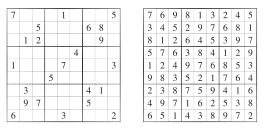
\includegraphics{sudoku.pdf}
        \caption{Sudoku Game and its solution\footnote{\tiny Elizabeth Arnold, Stephen Lucas, and Laura Taalman. \Grob basis representations of sudoku}}
        \label{fig:sudoku}
    \end{figure}
\end{frame}
\begin{frame}[allowframebreaks]{Sudoku}{Formulation and Modelling}
    \begin{itemize}
        \item The objective is to fill a $m\times m$ grid ($m=n^2$) with integers from $1$ to $m$ such that no row or column or block has a same number appear twice.
 \item Any such board, can be represented in the block matrix form with its each entry being a \emph{block} of dimension $n\times n$.
 \item We model a sudoku using Boolean Polynomials by creating $m\cdot(m^2)=m^3$ variables.
 \item $m$ boolean variables for every element of the grid.
 \item Let these variables be denoted by $x_{i,j}$ where $0\leq i\leq m^2-1$ and $0\leq j \leq m-1$, where $i$ represents the element number and $j$ represents the value that element can take
    \end{itemize}
    \end{frame}
    \begin{frame}{Sudoku}{Representation}
There are three kinds of polynomial equations to be created to denote the following conditions,
\begin{itemize}
    \item For every $i$, exactly one of $x_{i,j}$ must be 1. This is achieved using following,
    \begin{equation}
        \begin{aligned}
            \forall i, \sum_{j=0}^{m-1}\prod_{k\neq j} x_{i,k} &= 0 \text{ (for each $i$, $x_{i,j} = 0$ for atleast $m-1$\ $j$'s)}\\
            \forall i, \sum_{j=0}^{m-1} x_{i,j} &= 1 \text{ (for each $i$, not all $x_{i,j} = 0$) }
        \end{aligned}
    \end{equation}
    \item For $i_1,i_2$ such that they are in same row or column or block, they should not have the same number.
    \begin{equation}
        \sum_{j=0}^{m-1} x_{i_1,j}\cdot x_{i_2,j} = 0 \text{ (for all valid  $(i_1, i_2)$ pairs)}
    \end{equation}
    \item Encode the given value, if $x_i$ is $k$ then $x_{i,j}=1$ iff $j==k-1$. (i.e., other $x_{i,j}=0$)
\end{itemize}
\end{frame}
\begin{frame}{Sudoku}{Solution}
\begin{itemize}
    \item Create an ideal and add all the equations to it as polynomials and find its \Grob basis $G$.

\item If the system has no solution then $G=\{1\}$, else the polynomials of $G$ are in eliminated form.
\item If $G$ contains $m^3$ polynomials then there is a unique solution since each of the $m^3$ variable will have it's own linear equation (as $x^2=x$ for binary numbers) which is $x=0$ or $x+1=0$.
\item If $G$ contains less than $m^3$ polynomials  but more than one then $x$'s can be both $0$ or $1$ and $x$ is either eliminated from the equation or it is uniquely dependent on other variables which are eliminated at a later stage.
\end{itemize}
\end{frame}
\begin{frame}{Sudoku}
\href{https://github.com/paramrathour/Groebner-Basis-Applications/blob/main/Sudoku Solver.ipynb}{SageMath Demo}.
\end{frame}
\begin{frame}{Conclusion}
\begin{itemize}
\item \textbf{NP-hard} to compute and generated \Grob Basis have polynomials of higher degrees and larger coefficients. 
\item Applications designed for Solving Polynomial Equations, Lagrange Optimizations. Check \href{https://github.com/paramrathour/Groebner-Basis-Applications}{here}
\item More possible applications Vertex Coloring, Design of Computer Algebra Systems, Coding Theory are developed.
\item Future Directions on Fast Computations of \Grob Basis: Faugère's \href{https://www-polsys.lip6.fr/~jcf/Papers/F99a.pdf}{F4} and \href{https://www-polsys.lip6.fr/~jcf/Papers/F02a.pdf}{F5} algorithms and more application-specific development such as, \href{https://www.sciencedirect.com/science/article/pii/S0747717109000273}{PolyBoRi}, a \Grob basis framework for Boolean polynomials.
\end{itemize}
\end{frame}
\appendix
\section{References}
% \begin{frame}[allowframebreaks]
\begin{frame}[allowframebreaks]
  \frametitle<presentation>{References}
%   \bibliographystyle{plainnat}    
\bibliographystyle{plainurl}
  \nocite{*}
  {\bibliography{references}}
%   \begin{thebibliography}{10}
    
%   \beamertemplatebookbibitems
%   % Start with overview books.

%   \bibitem{Author1990}
%     A.~Author.
%     \newblock {\em Handbook of Everything}.
%     \newblock Some Press, 1990.
 
    
%   \beamertemplatearticlebibitems
%   % Followed by interesting articles. Keep the list short. 

%   \bibitem{Someone2000}
%     S.~Someone.
%     \newblock On this and that.
%     \newblock {\em Journal of This and That}, 2(1):50--100,
%     2000.
%   \end{thebibliography}
\end{frame}
\end{document}